\subsection{Wasserstoff Günstig Szenario - 5}

\subsubsection{Kenngrößen Szenario}

\captionof{table}{\label{table_5_kenngrößen_scenario} Basiskenngrößen Szenario 5}
\begin{center}
	\begin{tabularx}{\textwidth}{l | X } Kenngröße & Wert \\
	\hline
	Anzahl Untersuchungsgebiete & \num{155} \\
	Summe Streckenkilometer & \SI{13490}{\km} \\
	\ce{CO2}-Bilanz Ausgangssituation & \SI{6840168}{\tonne} \ce{CO2} \\
	\ce{CO2}-Bilanz Szenario 5 & \SI{168638}{\tonne} \ce{CO2}\\
	\end{tabularx}
\end{center}

\subsubsection{Kenngrößen Untersuchungsgebiete}
\captionof{table}{\label{table_5_kenngrößen_untersuchungsgebiete} Anzahl Untersuchungsgebiete sowie Kilometer nach Traktion 5}
\begin{center}
	\begin{tabularx}{\textwidth}{X | r | r | r} Traktion & Anzahl & Kilometer Infrastruktur & Betriebskilometer (pro Tag) \\
	\hline
            electrification & \num{27} &  \SI{420}{\km} & \SI{3824508}{\km}\\
            efuel & \num{0} &  \SI{0}{\km} & \SI{0}{\km}\\
            battery & \num{97} &  \SI{5936}{\km} & \SI{11398628}{\km}\\
            optimised electrification & \num{31} &  \SI{7134}{\km} & \SI{19927068}{\km}\\
            diesel & \num{0} &  \SI{0}{\km} & \SI{0}{\km}\\
            h2 & \num{0} &  \SI{0}{\km} & \SI{0}{\km}\\
            no calculated cost & \num{0} &  \SI{0}{\km} & \SI{0}{\km}\\
    	\end{tabularx}
\end{center}

\captionof{table}{\label{table_5_kenngrößen_untersuchungsgebiete_no_optimised} Anzahl Untersuchungsgebiete sowie Kilometer nach Traktion (Optimierte Elektrifizierung aufgeteilt) Szenario 5}
\begin{center}
	\begin{tabularx}{\textwidth}{X | r | r | r} Traktion & Anzahl & Kilometer Infrastruktur & Betriebskilometer \\
	\hline
            electrification & \num{27} &  \SI{3314}{\km} & \SI{16415616}{\km}\\
            efuel & \num{0} &  \SI{0}{\km} & \SI{0}{\km}\\
            battery & \num{97} &  \SI{10176}{\km} & \SI{18734588}{\km}\\
            diesel & \num{0} &  \SI{0}{\km} & \SI{0}{\km}\\
            h2 & \num{0} &  \SI{0}{\km} & \SI{0}{\km}\\
            no calculated cost & \num{0} &  \SI{0}{\km} & \SI{0}{\km}\\
    	\end{tabularx}
\end{center}
In dieser Tabelle wurden die Infrastrukturkilometer der Untersuchungsgebiete, bei denen die optimierte Elektrifizierung am wirtschaftlichsten war, auf die Traktionen Elektrifizierung und Batterie aufgeteilt (je nachdem, bei welchem Teiluntersuchungsgebiet welche Traktion am wirtschaftlichsten war)

\subsubsection{Kenngrößen Kosten}

\captionof{table}{\label{table_5_kenngrößen_investition} Basiskenngrößen Kosten 5}
\begin{center}
	\begin{tabularx}{\textwidth}{X | r } Kenngröße & Kosten [Barwert] \\
	\hline
	Investitionskosten & \num{6685443} Tsd. €\\
	Betriebskosten & \num{39485076} Tsd. €
	\end{tabularx}
\end{center}

\captionof{table}{\label{table_5_kenngrößen_investition_cost_by_traction} Investitionsvolumen sowie Betriebskosten (Barwert Preisstand 2016) Szenario 5}
\begin{center}
	\begin{tabularx}{\textwidth}{X | r | r} Traktion & Kosten Infrastruktur Barwert & Betriebskosten Barwert\\
	\hline
            electrification & \num{679388} Tsd. € &  \num{3490008} Tsd. €\\
            efuel & \num{0} Tsd. € &  \num{0} Tsd. €\\
            battery & \num{412736} Tsd. € &  \num{13094172} Tsd. €\\
            optimised electrification & \num{5593320} Tsd. € &  \num{22900896} Tsd. €\\
            diesel & \num{0} Tsd. € &  \num{0} Tsd. €\\
            h2 & \num{0} Tsd. € &  \num{0} Tsd. €\\
            no calculated cost & \num{0} Tsd. € &  \num{0} Tsd. €\\
    	\end{tabularx}
\end{center}

\begin{center}
	\begin{figure}[p]
	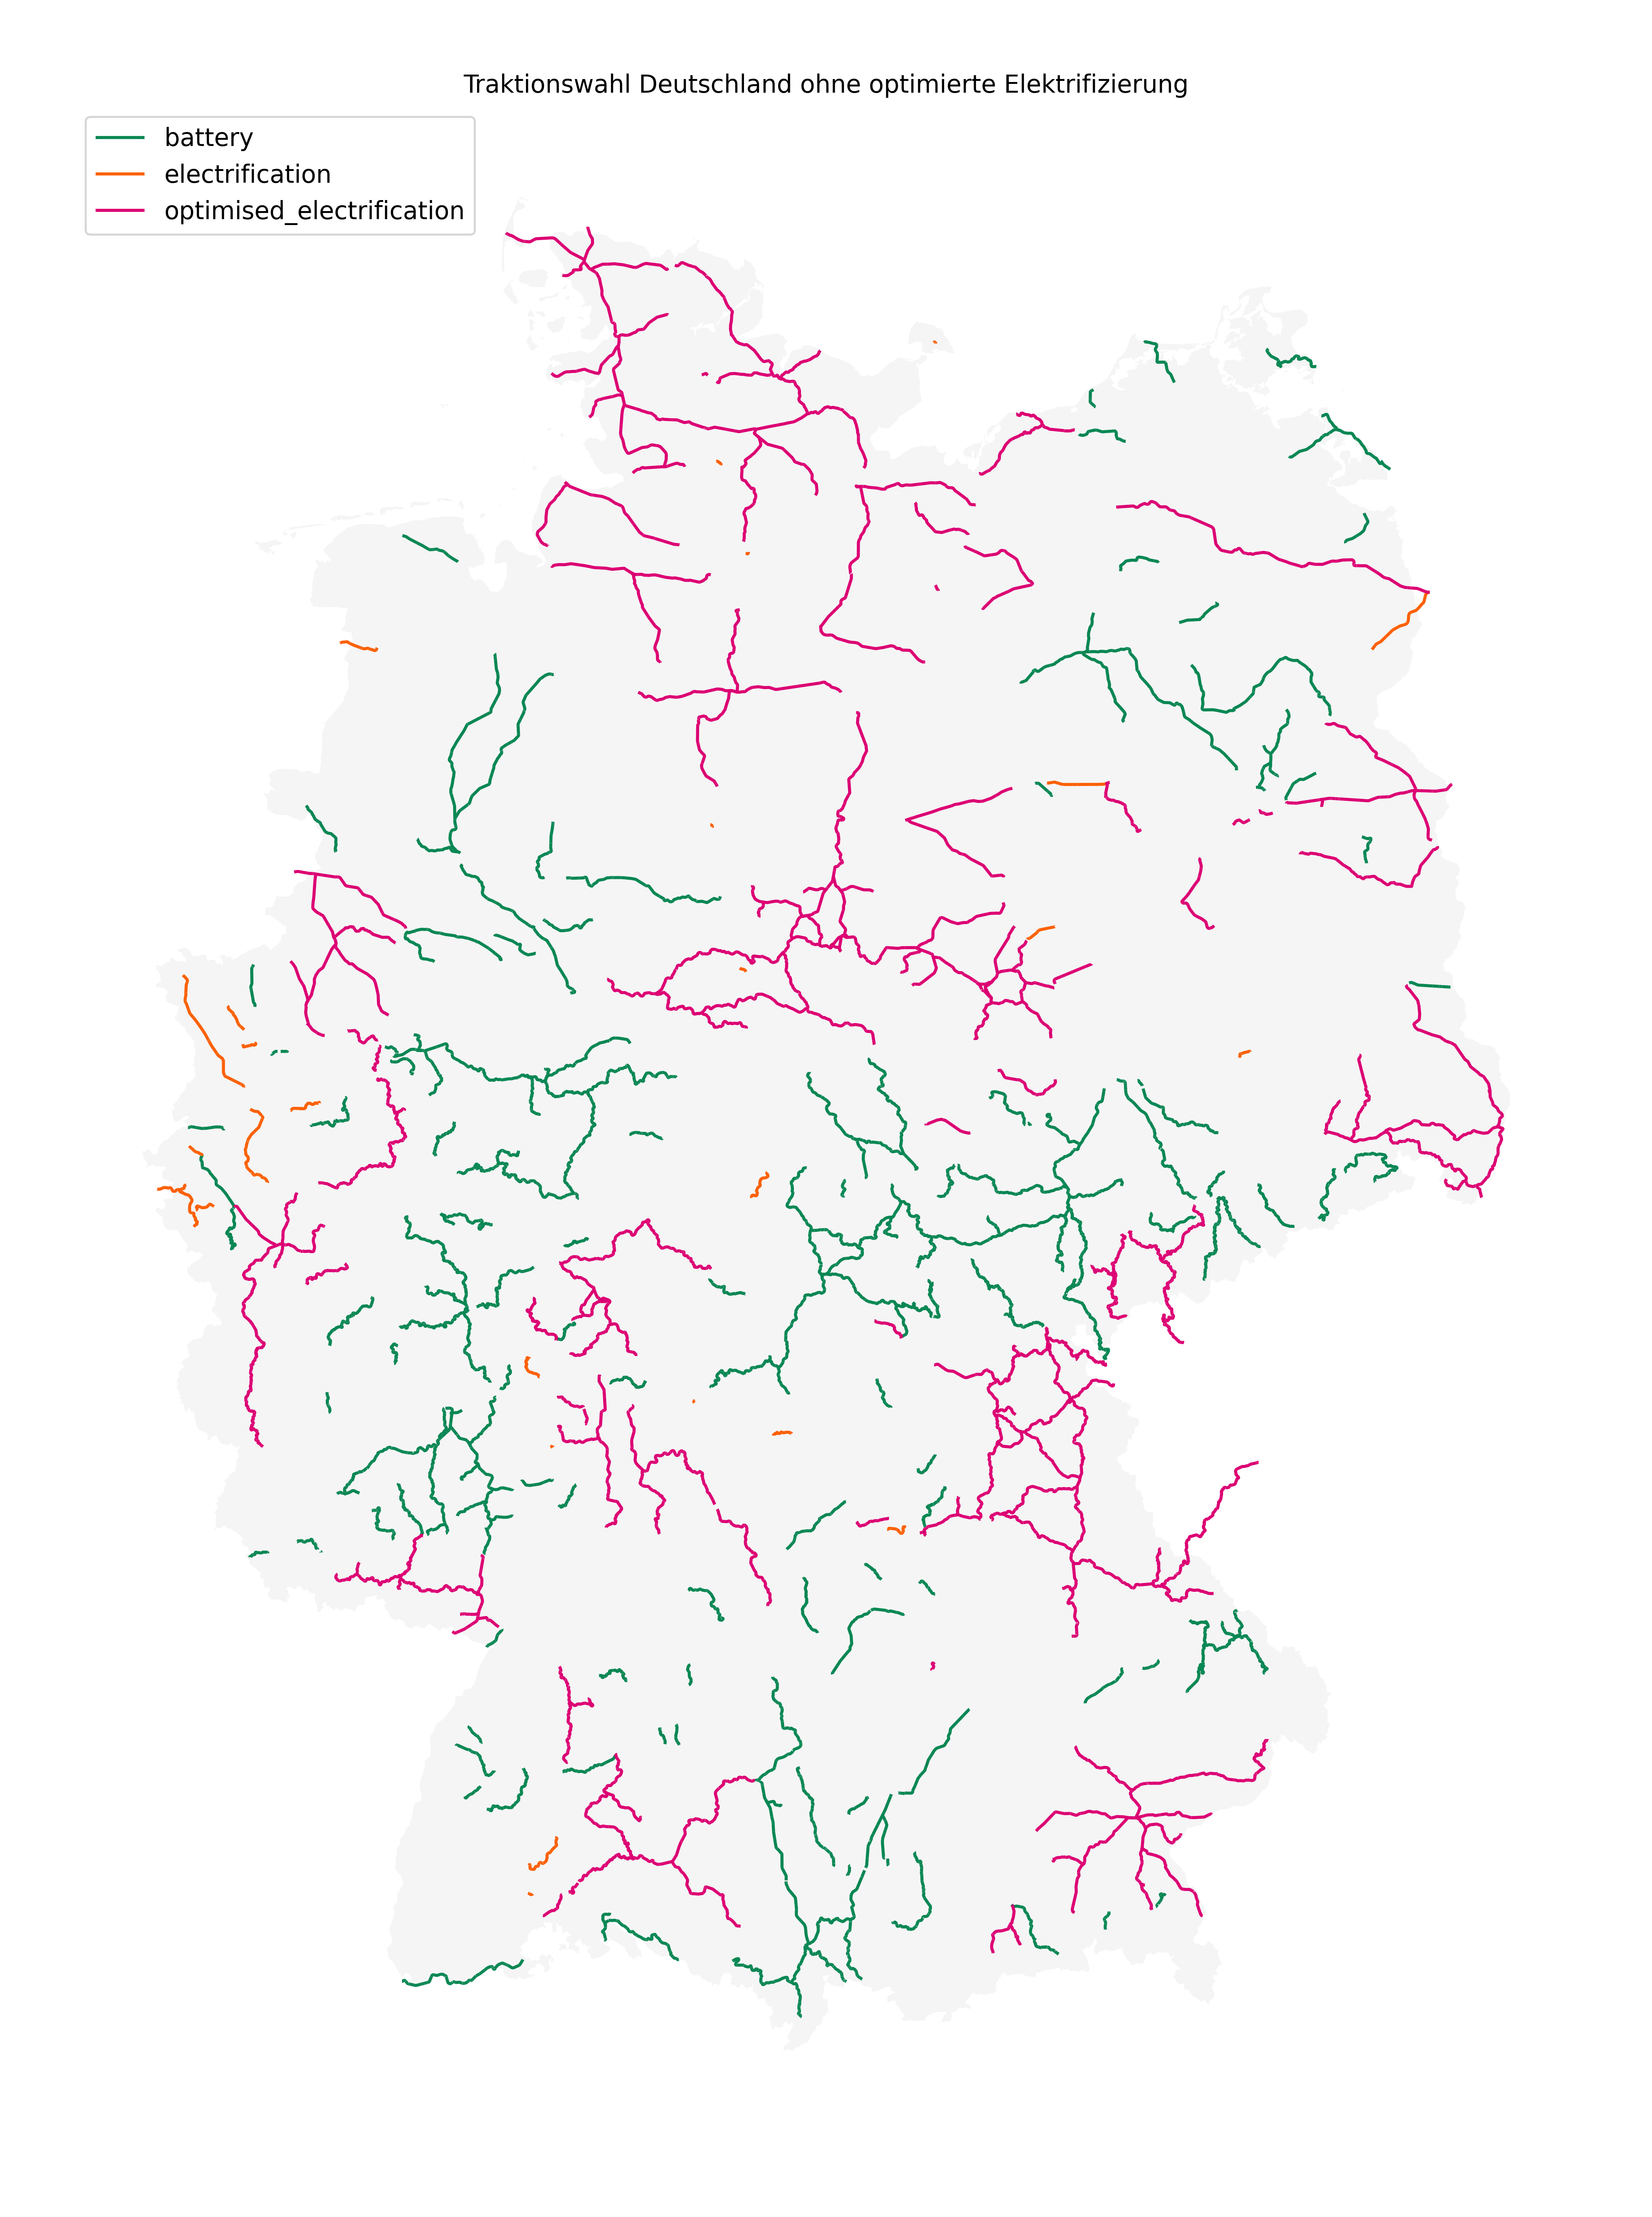
\includegraphics[height=0.8\textheight]{../report_scenarios/s_5/files/deutschland_map}
	\caption{\label{fig_s_5_d_map} Karte Deutschland bevorzugte Traktion Untersuchungsgebiete Szenario 5}
	\end{figure}
\end{center}

\newpage
\subsubsection{Kenngrößen \acrlong{sgv}}
\captionof{table}{\label{table_5_kenngrößen_sgv} Kenngrößen \acrlong{sgv} 5}
\begin{center}
	\begin{tabularx}{\textwidth}{l | X } Kenngröße & Wert \\
	\hline
	Betriebsleistung \acrshort{sgv} (Linien mit Abschnitten ohne Oberleitung) & \num{130993.21200000006}
	\end{tabularx}
\end{center}